\chapter{A Comparison of Melanoma Segmentation Algorithms using Neural Networks and Statistical Models}

\section{Introduction}
This section includes a discussion on segmentation techniques for the detection of melanoma. The goal is to produce a statistically significant border cut-off at the perimeter of the skin lesion. An accurate border cut-off is an essential criterion for melanoma detection\cite{Pereira2020, Kaya2016} using ABCD rules. Unfortunately, segmentation continues to be a challenging task because datasets regularly contain an estimated border and sometimes an inaccurate border cut-off. This chapter includes a simple border analysis technique called fractal box-counting to assess the benefits of using segmentation algorithms with accurate border cut-offs.

\section{Related Works}
An approach by Albanhli\cite{Albahli2020} uses a deep learning-based segmentation algorithm using YOLOv4-arkNet and active contouring for melanoma and skin lesion detection and segmentation. This technique provides a classification of the skin lesion and a segmentation, demonstrating a high level of practicality for clinical decision support systems. 

Seeja R D\cite{seeja2019} proposed a technique that utilizes a convolutional neural network (CNN) based on a U-net model architecture for the segmentation based on colour, texture and shapes. The U-net model architecture is a popular choice for image segmentation tasks due to its ability to capture both local and global features effectively.

Hyunju Lee\cite{Lee2020} proposed a technique that utilizes an edge fill method called u-otsu for segmentation, using the U cahnnel from the YUV colour space to calculate the histogram. Otsu calculates the optimal threshold value to separate foreground and background pixels based on the histogram of the image.

Another technique by Pedro\cite{Pereira2020} uses a newly developed technique called Local Binary Patterns Clustering (LBPC). Using a Local Binary Pattern (LBP) filter by subtracting the grayscale image from the LBP filter after a Gaussian filter, resulting in the creation of a mask. This has been successfully used for the detection of melanoma.

\section{Skin Lesion Segmentation}
Segmentation plays a crucial role in melanoma detection because it separates melanoma from healthy skin. Accurate segmentation is essential for various aspects of melanoma diagnosis and treatment, and classification\cite{Albahli2020} including improving the detection of of ABCD rules\cite{Lee2020}. One of the important features is border, 

A range of traditional segmentation techniques including SegNet, U-net methods have been shown to outperform other approaches in capturing the most significant melanoma characteristics. However, these techniques do not provide an effective border for the analysis of ABCD rules. Other techniques have been explored including active countouring-based segmenatation\cite{Riaz2019}, LBPC and others for border adjustment include u-otsu and edge-imfill.


\subsection{Semantic Pixel Wise Segmentation (SegNet)}
SegNet is a deep learning architecture that is used for semantic image segmentation for melanoma detection. It was originally developed by\cite{chen2018} and has shown promising results in various segmentation tasks.

The idea of SegNet is to perform pixel-wise classification by assigning each pixel in an image to a specific class or category. This is achieved through a fully convolutional neural network (FCN) architecture, which allows for end to end learning and inference at the pixel level. 

Semantic pixel-wise segmentation (SegNet) is a machine learning architecture utilizing a deep, fully convolutional neural network (DCNN). This network requires training from ground-truth and pre-segmented images for automatic segmentation. SegNet consists of encoding layers, decoding layers, and a pixel-wise classification layer. The encoder layers consist of 3x3 convolutions (including batch normalization and ReLU), pre-trained filters for classifying features. After some convolutions, the data is down-sampled using a 2x2 pooling layer. Next, decoding layers consist of up-sampling, followed by 3x3 convolutions. Finally, the pixel-wise classification uses a softmax layer to represent each pixel between 0 and 1 based on the previous layers, generating a segmentation mask.

\begin{figure}[hb]
\centering
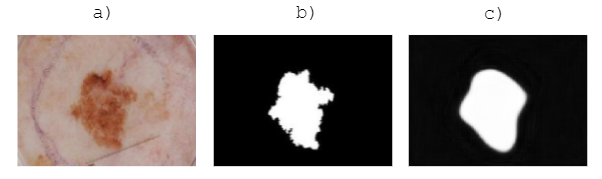
\includegraphics[scale=1.2]{images/border-seg.png}
\caption{Demonstrating the Semantic Pixel-Wise Segmentation (SegNet) results showing the a) original image, b) expert ground-truth and c) SegNet results.} \label{SegNet}
\end{figure}

Results in figure \ref{SegNet} are generated from the architecture using the ISIC 2018 dataset split into 80\% training and 20\% validation images. The accuracy of locating the lesions is 85\%. However, figure \ref{SegNet} represents the border cut-off between skin and skin lesion is accurate to the dataset but inadequate for using the ABCD rules. Finding the border cut-off is vital for measuring ABCD rules\cite{Pereira2020}.

\section{Border extraction}
To prove the usefulness of segmentation techniques with an accurate border cut-off a technique developed by Ali\cite{Ali2020b} is implemented that utilises machine learning with extracted data including Zernike moments, fractal box-counting, and convexity measurements. Fractal box-counting is used to measure the irregularity of the border.

The fractal box-counting technique is a commonly employed technique for analysing fractal properties. It involves dividing a fractal object or pattern into a grid of equally sized boxes and counting the number of boxes that contain a portion of the fractals. The process is repeated with different box sizes until the boxes until relationship between the box sizes and number of boxes is analysed determining the fractal dimension\cite{Hamburger1996}. Essentially a more complicated border with corners and convexes will have more boxes and therefore a higher fractal score, than for example a border with smooth corners and edges which has a lower score. This should provide some evidence on the usefulness of an accurate border.

\subsection{U-Otsu Threshold}
Otsu threshold is a versatile automatic image thresholding technique meant to separate each pixel between two classes of foreground or background. One of the benefits of this method is that it does not require any training data. The equation \ref{otsu} (within-class variance) describes splitting weights of $w_0(t),w_1(t)$, which are the probabilities divided by the threshold $t$, between 0 to 255. Furthermore, $\sigma_1^2$ and $\sigma_0^2$ are variances of these two classes. The class probability $w$ is computed from the histogram in figure \ref{otsu2}, which is an intensity histogram describing the colour distribution in an image. Measuring the values above and below the generated thresholds splits the image into two classes.

\begin{equation} \label{otsu}
\sigma_w^2(t) = w_0(t)\sigma_1^2(t) + w_1(t)\sigma_2^2(t)
\end{equation}

The histogram is split into two segments with the threshold $t$ of 138 and the corresponding pixel locations to the histogram segment the skin lesion into two classes. Image morphology closing is applied to fill gaps that the threshold missed. On other occasions, the segmentation missed the skin lesion because of a similar colour between the skin and skin lesion. It might be beneficial to combine otsu with SegNet to improve its accuracy while producing a border cut-off. Figure \ref{otsu2} describes the difference between otsu and SegNet.

\begin{figure}
\centering
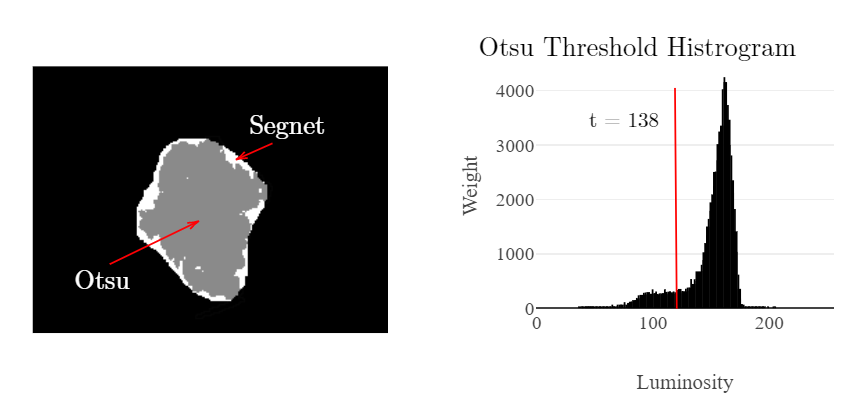
\includegraphics[scale=0.7]{images/otsu3.png}
\caption{Otsu thresholding alongside ground-truth mask, where grey Otsu and white is SegNet. The bar chart shows the histogram with an otsu threshold of 138.} \label{otsu2}
\end{figure}


\subsection{LBPC segmentation}

Local Binary Patterns (LBP) is a texture descriptor commonly used for augmenting the image improving classification accuracy\cite{Pereira2020, Kaya2016}. First, equation\ref{eq1} calculates each pixel, where $p$ (equal to 8) is the number of neighbouring pixels compared to the centre of $c$, and the radius of $r$ from the centre. Next, shown in equation\ref{eq2} each value is subtracted counter-clockwise with the centre value and compared to function $S$ where each $gp - gc$, if more than or equal to 0, is equal to 1, and less than 0 is equal to 0. Next, add corresponding values equal to 1 of $gp$ together, changing the centre value, ignoring values of 0. Next, applying a Gaussian kernel of 13-pixel iterations and a standard deviation of 3 removes smaller features that interfere with the segmentation. Finally, applying k-means with a value of 2 subtracts the greyscale and segments the skin lesion from the skin.

\begin{equation} \label{eq1}
LBP(gp_x, gp_y) = \mathlarger{\sum}_{p=0}^{P-1}s\big(gp - gc)2^p
\end{equation}

\begin{equation} \label{eq2}
s\big(x) = 
\begin{cases}
1,\:\:x\geq\:0; \\
0,\:$otherwise$.
\end{cases}
\end{equation}

Figure \ref{fractal1} demonstrates the segmentation of two skin lesions, one with an irregular border and another with a regular border. LBPC is applied to both skin lesions, followed by Gaussian blurring and morphology closing to remove dots. The result is an improved border cut-off compared to the ground-truth in the Ph$^2$ dataset with more corners and ledges. This technique will improve accuracy for measuring border irregularity\cite{Pereira2020}.

\begin{figure}
\centering
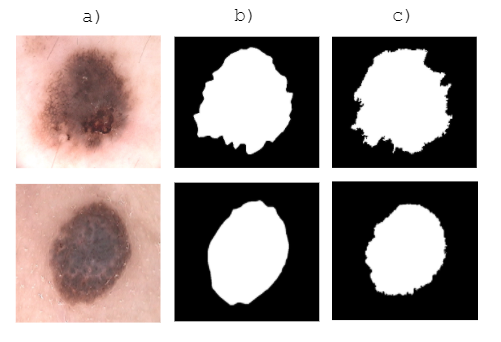
\includegraphics[scale=1.2]{images/borders.PNG}
\caption{Local Binary Pattern Clustering (LBPC) showing the a) original image, b) ground-truth, and c) LBPC. LBPC successfully exaggerates the border cut-off on the skin lesions with regular and irregular borders} 
\end{figure} \label{fractal1}

Validating LBPC is not expected because the goal is to exaggerate the border to improve the classification process of ABCD rules, which it does successfully\cite{Pereira2020, Kaya2016}. For example, the segmentation might not match dataset segmentations but is still essential to classifying ABCD rules. Furthermore, many datasets lack expert border segmentation, an accurate border cut-off between the skin and skin lesions, so comparisons are not always possible.

\section{Comparison of techniques}
Overall the accuracy of the techniques demonstrates that SegNet is the most reliable technique. However, comparing the techniques in \ref{} we can demonstrate that it produces a smudge effect and fails to capture the border cut-off from the skin lesion, but it is successful at finding the location of the skin lesion.

Both statistical models of LBPC and Otsu threshold generated an accurate border cut-off between the skin and the skin lesion As previously mentioned, measuring the border cut-off and exaggerating irregular borders are helpful when calculating the ABCD rules. 

It might be beneficial to combine SegNet and LBPC using SegNet to find the skin lesions' location, followed by adjusting the border cut-off using LBPC. A similar technique using the Otsu threshold and Segnet is described by\cite{Riaz2019}.

\section{Joint Neural network and statistcal model approach}
